\documentclass{article}
\usepackage{fullpage}
\usepackage{indentfirst}
\usepackage{amsmath}
\usepackage{amsfonts}
\usepackage{array}
\usepackage{tipa}
\usepackage{tikz}
\usepackage{tikz-qtree}
\usetikzlibrary{matrix, arrows, automata}
\usepackage{gb4e}
\noautomath
\newcommand{\Y}{$\checkmark$}
\newcommand{\N}{\ding{55}}
\newcommand{\R}{$\Rightarrow$}
\newcommand\myeq{\mathrel{\stackrel{\makebox[0pt]{\mbox{\normalfont\tiny def}}}{=}}}
\title{Representations: Yip (1989) vs Bao (1990) [Revisions]}
\author{Chris Oakden}
\begin{document}
\maketitle
\section{New stuff}
New Definitions of models, specifically making association non-reflexive. \\
Yip's model:
\begin{equation}
\begin{split}
\mathcal{M}^{Y'}_{H} = \langle \mathcal{D}; &P_{\sigma}, P_{+u}, P_{h}, \alpha(x), \delta(x) \rangle \\
\mathcal{D} &= \{1, 2, 3\} \\
P_{\sigma} &= \{1\} \\
P_{+u} &= \{2\} \\
P_{h} &= \{3\} \\
\alpha(x) &= \begin{cases} 2 & x=1 \end{cases} \\
\delta(x) &= \begin{cases} 3 & x = 2 \end{cases} 
\end{split}
\end{equation}
Bao's model: \\
\begin{equation}
\begin{split}
\mathcal{M}^{B'}_{H} = \langle \mathcal{D}; P_{\sigma}, P_{T}, &P_{+u}, P_{c}, P_{h}, \alpha(x), \delta(x) \rangle \\
\mathcal{D} &= \{1, 2, 3, 4, 5\} \\
P_{\sigma} &= \{1\} \\
P_{T} &= \{2\} \\
P_{+u} &= \{3\} \\
P_{c} &= \{4\} \\
P_{h} &= \{5\} \\
\alpha(x) &= \begin{cases} 2 & x=1 \end{cases} \\
\delta(x) &= \begin{cases} 2 & x\in\{3,4\} \\
				     4 & x=5 \end{cases} \\
\end{split}
\end{equation}
The transduction from $\mathcal{M}^{B'}_{H}$ to $\mathcal{M}^{Y'}_{H}$ ($\tau^4$) is thus:
\begin{equation} \label{tau4}
\begin{split}
&\tau^4 \\
P^{\tau^4}_{\sigma}(x) &\myeq P_{\sigma}(x) \\
P^{\tau^4}_{+u}(x) &\myeq P_{T}(x) \\
P^{\tau^4}_{h}(x) &\myeq P_{c}(x) \\
\alpha^{\tau^4}(x)=y &\myeq \alpha(x) \\
\delta^{\tau^4}(x) = y &\myeq \varphi(x,y)\,|\, P_{c}(x) \wedge P_{T}(y) \\
\end{split}
\end{equation}
As a graph transduction, $\tau^4$ will look like this (input on left, output on right): \\
\begin{center}
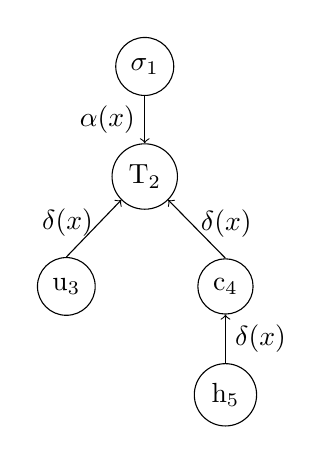
\begin{tikzpicture}
\matrix (m) [matrix of nodes, nodes={circle, draw, minimum size = .7cm}, column sep = .2cm, row sep = .6cm]{
& $\sigma_{1}$ & \\
& T$_2$ & \\
u$_3$ & & c$_4$\\
&&h$_5$\\
};
\draw [->] (m-1-2.south) -- (m-2-2.north) node[left, pos=.5]{$\alpha(x)$}; 
\draw [->] (m-3-1.north) -- (m-2-2.south west) node[left, text width=.6cm,pos=.6]{$\delta(x)$};
\draw [->] (m-3-3.north) -- (m-2-2.south east) node[right, text width=.6cm,pos=.6]{$\delta(x)$};
\draw [->] (m-4-3.north) -- (m-3-3.south) node[right, text width=.6cm,pos=.5]{$\delta(x)$};
\end{tikzpicture}
\hspace{2cm}
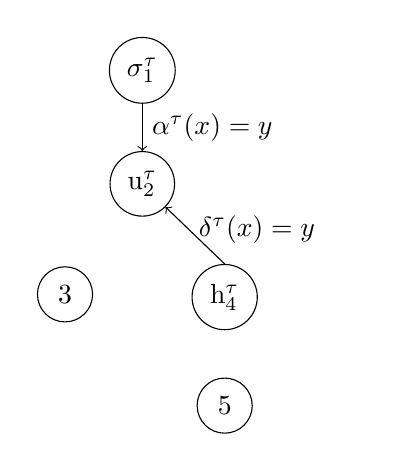
\begin{tikzpicture}
\matrix (m) [matrix of nodes, nodes={circle, draw, minimum size=.7cm}, column sep = .2cm, row sep = .6cm]{
& $\sigma^{\tau}_{1}$ & \\
& u$^{\tau}_2$ & \\
3 & & h$^{\tau}_4$\\
&&5\\
};
\draw [->] (m-1-2.south) -- (m-2-2.north) node[right, pos=.5]{$\alpha^{\tau}(x)=y$}; 
\draw [->] (m-3-3.north) -- (m-2-2.south east) node[right, text width=2cm,pos=.6]{$\delta^{\tau}(x)=y$};
\end{tikzpicture}
\end{center}
For the transduction from $\mathcal{M}^{Y'}_{H}$ to $\mathcal{M}^{B'}_{H}$ ($\tau^3$), we set k = 2. \\
\begin{equation}
\begin{aligned}
P^1_{\sigma}(x) &\myeq P_{\sigma}(x) &  P^2_{\sigma}(x) &\myeq \mathtt{False} \\
P^1_{T}(x) &\myeq P_{+u}(x) &  P^2_{T}(x) &\myeq \mathtt{False} \\
P^1_{+u}(x) &\myeq P_{h}(x) &  P^2_{+u}(x) &\myeq \mathtt{False} \\
P^1_{c}(x) &\myeq \mathtt{False} &  P^2_{c}(x) &\myeq P_{\sigma}(x) \\
P^1_{h}(x) &\myeq \mathtt{False} &  P^2_{h}(x) &\myeq P_{+u}(x) \\
\alpha^{1,1}(x)=y &\myeq \alpha(x) & \alpha^{1,2}(x)=y &\myeq \mathtt{False}  \\
\alpha^{2,1}(x)=y &\myeq \mathtt{False} & \alpha^{2,2}(x)=y &\myeq \mathtt{False}  \\
\delta^{1,1}(x)=y &\myeq \delta(x) & \delta^{1,2}(x)=y &\myeq \mathtt{False}  \\
\delta^{2,1}(x)=y &\myeq \varphi(x,y) | P_{\sigma}(x) \wedge P_{+u}(y) & \delta^{2,2}(x)=y &\myeq \varphi(x,y) | P_{h}(x) \wedge P_{+u}(y)  \\
\end{aligned}
\end{equation} \\
The graph transduction for $\tau^3$ would look like:
\begin{center}
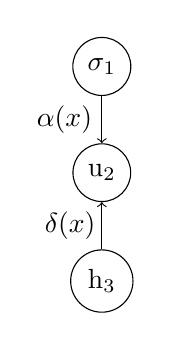
\begin{tikzpicture} [baseline = (m-1-1.base)]
\matrix (m) [matrix of nodes, nodes={circle, draw, minimum size=.7cm}, column sep = .2cm, row sep = .6cm]{
$\sigma_{1}$ \\
u$_{2}$ \\
h$_{3}$ \\
};
\draw [->] (m-1-1.south) -- (m-2-1.north) node[left, pos=.5]{$\alpha(x)$};
\draw [->] (m-3-1.north) -- (m-2-1.south) node[left, text width=.6cm,pos=.5]{$\delta(x)$};
\end{tikzpicture}
\hspace{3cm}
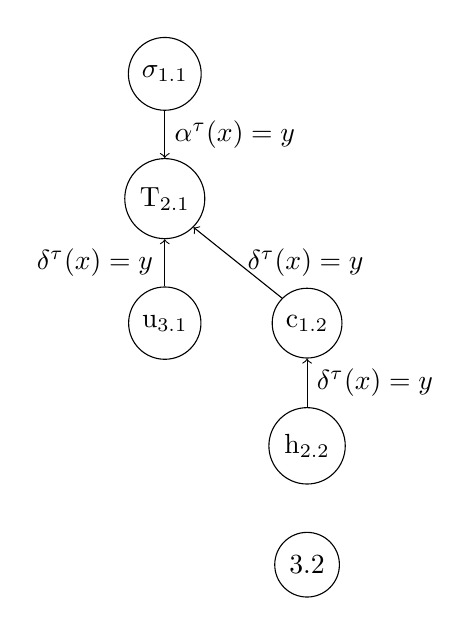
\begin{tikzpicture} [baseline = (m-1-1.base)]
\matrix (m) [matrix of nodes, nodes={circle, draw, minimum size=.7cm}, column sep = .8cm, row sep = .6cm]{
$\sigma_{1.1}$ & \\
T$_{2.1}$ & \\
u$_{3.1}$ & c$_{1.2}$  \\
& h$_{2.2}$ \\
& 3.2 \\
};
\draw [->] (m-1-1.south) -- (m-2-1.north) node[right, pos=.5]{$\alpha^{\tau}(x)=y$};
\draw [->] (m-3-1.north) -- (m-2-1.south) node[left, text width=1.5cm,pos=.5]{$\delta^{\tau}(x)=y$};
\draw [->] (m-3-2.north west) -- (m-2-1.south east) node[right, text width=1.5cm,pos=.5]{$\delta^{\tau}(x)=y$};
\draw [->] (m-4-2.north) -- (m-3-2.south) node[right, text width=1.5cm, pos=.5]{$\delta^{\tau}(x)=y$};
\end{tikzpicture}
\end{center}
\newpage
Let's unpack this a bit. The syllable node in the first copy set of the output structure corresponds to the input syllable position. It is therefore set to false in the second copy set. The tonal root node `T' in the first copy set is equivalent to the register node [+u] in the input, and is also false in the second copy set. The position of the output register node corresponds to the terminal root node in the input structure (and is again false in the second copy set). The contour and tonal root nodes (part of the second copy set) are defined in terms of the input syllable and register nodes, respectively.\par
Going from the first copy set to the first copy set, both association and dominance functions are preserved. No first copies associate with second copies. Second copies associate with neither first nor second copies, so the output functions $\alpha^{1,2}(x)$, $\alpha^{2,1}(x)$, and $\alpha^{2,2}(x)$ are all set to false. Two additional dominance relations are needed, one between the second and first copy sets to capture $\delta$(c,T), and the other within the second copy set ($\delta$(h,c)). These are defined with respect to input structure positions across or within copy sets, $P_{\sigma}(x)_{2}\mapsto P_{+u}(x)_{1}$ and $P_{+u}(x)_{2}\mapsto P_{\sigma}(x)_{2}$ respectively.
\section{The General Model}
Let's create general models of Yip and Bao tonal geometry, and of transduction between the two. Generalizing the models borrows heavily from Kristina's Berber paper. \par
What we want to formalize first is the notion that the register node can be specified as either \textbf{High} register ([+stiff vocal chords] in Bao and [+upper] in Yip) or \textbf{Low} register ([-stiff vocal chords] in Bao and [-upper] in Yip). Similarly, the terminal tonal nodes (dominated by the `c' node in Bao and dominated by register in Yip) can be specified as either `\textbf{h}' ([-slack] for Bao, [+raised] for Yip) or `\textbf{l}' ([+slack] for Bao, [-raised] for Yip). We can thus specify two sets of features: register features ($\mathcal{RF}$) and contour features ($\mathcal{CF}$). Each set contains two members.
\begin{align}
\mathcal{RF} &\myeq \{+u, -u\} \\
\mathcal{CF} &\myeq \{h, l\}
\end{align}
For each member of the respective sets, there is a unary relation that labels a domain element with that feature. Let $\mathcal{P}_{rf}$ and $\mathcal{P}_{cf}$ be the sets of those unary relations.
 \begin{align}
 \mathcal{P}_{rf} &\myeq \{P_{rf}\,|\,rf \in \mathcal{RF}\} \\
 \mathcal{P}_{cf} &\myeq \{P_{cf}\,|\,cf \in \mathcal{CF}\}
 \end{align}
The node designating the TBU (in this case the syllable) can be defined in a similar way. Let $\mathcal{P}_{tbu}$ be the singleton set containing the unary relation $P_{\sigma}$. \par
The general Yip model $\mathfrak{M}^Y$ is thus defined as:
\begin{equation}
\mathfrak{M}^{Y} \myeq \langle\mathfrak{D}; \{\mathcal{P}_{rf}\cup\mathcal{P}_{cf}\cup\mathcal{P}_{tbu}\};\{\alpha(x), \delta(x)\}\rangle
\end{equation}
The general Bao model is very much the same, with the addition of individual unary relations for labelling the `T' and `c' nodes:
\begin{equation}
\mathfrak{M}^{B} \myeq \langle\mathfrak{D}; \{\mathcal{P}_{rf}\cup\mathcal{P}_{cf}\cup\mathcal{P}_{tbu}\cup P_{T}\cup P_{c}\};\{\alpha(x), \delta(x)\}\rangle
\end{equation} 
What do the association and dominance functions look like in the general models? In Yip's model, the TBU associates so the root node, in this case the register node. And the terminal node is dominated by the register node. Thus, we have:
\begin{equation}
\begin{aligned}
\alpha(x) \myeq \begin{cases} P_{rf} & x = P_{\sigma} \end{cases} \qquad \delta(x) \myeq \begin{cases} P_{rf} & x = P_{cf} \end{cases}
\end{aligned}
\end{equation}
In Bao's model, the association function has the same definition. Generalizing the dominance function captures the fact that register and `c' nodes are always dominated by the root `T', and that terminal tone node(s) are always dominated by `c'.
\begin{equation}
\delta(x) \myeq \begin{cases} P_{T} & x \in \{P_{rf}, P_{c}\} \\
				         P_{c} & x = P_{cf} \end{cases}
\end{equation}
In theory, then, the general models work for both level and contour tones. Consider a falling tone model in Yip.
\begin{center}
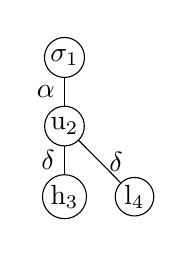
\begin{tikzpicture} [baseline = (x.base)]
\matrix (m) [matrix of nodes, column sep = 1em, row sep = 1em]{
\node[draw,circle, inner sep =1pt](x){$\sigma_{1}$}; \\
\node[draw,circle, inner sep =1pt](y){u$_{2}$}; \\
\node[draw,circle, inner sep =1pt](z){h$_{3}$}; & \node[draw,circle, inner sep =1pt](v){l$_{4}$}; \\
};
\draw (x) -- (y) node[left, pos=.5]{$\alpha$};
\draw (z) -- (y) node[left, pos=.5]{$\delta$};
\draw (v) -- (y) node[right, pos=.5]{$\delta$};
\end{tikzpicture}
\hspace{2cm}
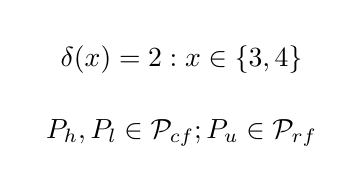
\begin{tikzpicture} [baseline = (m-1-1.base)]
\matrix (m) [matrix of nodes, align=left, column sep = 1pt, row sep = 1em]{
$\delta(x) = 2:x\in\{3,4\}$\\
$P_{h}, P_{l} \in \mathcal{P}_{cf}; P_{u} \in \mathcal{P}_{rf}$\\
};
\end{tikzpicture}
\end{center}
The definition of the dominance function follows the general definition since nodes which serve as the domain of the function \{3,4\} are labelled by the unary relations $P_{h}$ and $P_{l}$ respectively, both of which are in the set $\mathcal{P}_{cf}$. The codomain of the function is labeled by the relation $P_{+u}$, which is in the relation set $\mathcal{P}_{rf}$. The same generalizations can be inferred for Bao's model with nodes `T' and `c'
\begin{center}
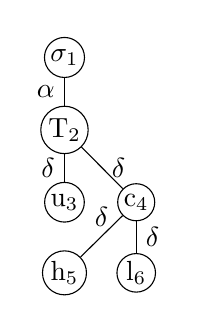
\begin{tikzpicture} [baseline = (x.base)]
\matrix (m) [matrix of nodes, column sep = 1em, row sep = 1em]{
\node[draw,circle, inner sep =1pt](x){$\sigma_{1}$}; \\
\node[draw,circle, inner sep =1pt](y){T$_{2}$}; \\
\node[draw,circle, inner sep =1pt](z){u$_{3}$}; & \node[draw,circle, inner sep =1pt](v){c$_{4}$}; \\
\node[draw,circle, inner sep =1pt](q){h$_{5}$}; & \node[draw,circle, inner sep =1pt](s){l$_{6}$}; \\
};
\draw (x) -- (y) node[left, pos=.5]{$\alpha$};
\draw (z) -- (y) node[left, pos=.5]{$\delta$};
\draw (v) -- (y) node[right, pos=.5]{$\delta$};
\draw (q) -- (v) node[above, pos=.5]{$\delta$};
\draw (s) -- (v) node[right, pos=.5]{$\delta$};
\end{tikzpicture}
\hspace{2cm}
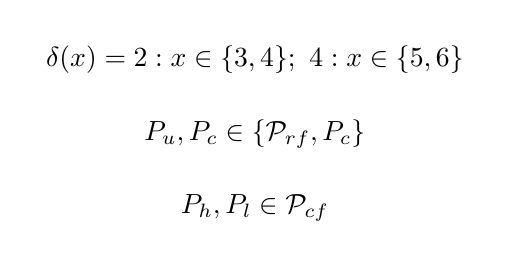
\begin{tikzpicture} [baseline = (m-1-1.base)]
\matrix (m) [matrix of nodes, align=left, column sep = 1pt, row sep = 1em]{
$\delta(x) = 2:x\in\{3,4\};\ 4:x\in\{5,6\}$\\
$P_{u}, P_{c} \in \{\mathcal{P}_{rf}, P_{c}\}$\\
$P_{h}, P_{l} \in \mathcal{P}_{cf}$\\
};
\end{tikzpicture}
\end{center}
\par
Now we can try to perform transductions on these models. A first pass at the general transduction $\Gamma_{\text{yb}}$ from Yip's model to Bao's model follows the specific transduction $\tau^4$ on high tone in (\ref{tau4}), but generalizes to any combination of register and single terminal tone features.
\begin{equation}
\begin{split}
P^{\Gamma}_{\sigma}(x) &\myeq P_{\sigma}(x) \\
P^{\Gamma}_{rf}(x) &\myeq P_{T}(x) \\
P^{\Gamma}_{cf}(x) &\myeq P_{c}(x) \\
\alpha^{\Gamma}(x)=y &\myeq \alpha(x)\\
\delta^{\Gamma}(x)=y &\myeq \varphi(x,y)\,|\,P_{c}(x)\land P_{T}(y)
\end{split}
\end{equation}
This definition is sufficient to translate any level tone in Yip's model to any level tone in Bao's model, that is, any of the four possible combinations of register and terminal node [+u, h], [+u, l], [-u, h], or [-u, l]. But will it work on contours? Probably not in the current state, as nodes with the contour feature labels (i.e. terminal tonal nodes) in the output model correspond to the `c' node in the input model, of which there is only one. Recall that `c' and `u' nodes are sisters in the input model (both dominated by the root node). We can exploit this to model contours in a Yip output model. Consider the appended general transduction $\Gamma_{\text{yb}}$ below:
\begin{equation}
\begin{split}
P^{\Gamma}_{\sigma}(x) &\myeq P_{\sigma}(x) \\
P^{\Gamma}_{rf}(x) &\myeq P_{T}(x) \\
P^{\Gamma}_{cf}(x) &\myeq P_{c}(x) \lor P_{rf}(x) \\
\alpha^{\Gamma}(x)=y &\myeq \alpha(x)\\
\delta^{\Gamma}(x)=y &\myeq \varphi(x,y)\,|\,\Big(P_{c}(x)\land P_{T}(y)\Big)\lor\Big(P_{rf}(x)\land P_{T}(y)\Big)
\end{split}
\end{equation}
A disjunct is added to the definition of terminal tonal nodes, as well as to the definition of the dominance function. The sum effect of these additions is the realization of contour tones without losing generalizability to level tones. Terminal level tones in the output can correspond to either the register or `c' node in the input structure and preserve structural integrity.
\begin{center}
\begin{tikzpicture}[baseline = (m-2-1.base)]
\matrix (m) [matrix of nodes, nodes={circle, draw, minimum size = .7cm}, column sep = .2cm, row sep = .6cm]{
& $\sigma_{1}$ & \\
& T$_2$ & \\
rf$_3$ & & c$_4$\\
&&cf$_5$\\
};
\draw [->] (m-1-2.south) -- (m-2-2.north) node[left, pos=.5]{$\alpha(x)$}; 
\draw [->] (m-3-1.north) -- (m-2-2.south west) node[left, text width=.6cm,pos=.6]{$\delta(x)$};
\draw [->] (m-3-3.north) -- (m-2-2.south east) node[right, text width=.6cm,pos=.6]{$\delta(x)$};
\draw [->] (m-4-3.north) -- (m-3-3.south) node[right, text width=.6cm,pos=.5]{$\delta(x)$};
\end{tikzpicture}
\hspace{.5cm}
$\rightarrow$
\hspace{.5cm}
\begin{tikzpicture} [baseline = (m-2-1.base)]
\matrix (m) [matrix of nodes, nodes={circle, draw, minimum size=.7cm}, column sep = .2cm, row sep = .6cm]{
& $\sigma^{\Gamma}_{1}$ & \\
& rf$^{\Gamma}_2$ & \\
3 & & cf$^{\Gamma}_4$\\
&&5\\
};
\draw [->] (m-1-2.south) -- (m-2-2.north) node[right, pos=.5]{$\alpha^{\Gamma}(x)=y$}; 
\draw [->] (m-3-3.north) -- (m-2-2.south east) node[right, text width=2cm,pos=.6]{$\delta^{\Gamma}(x)=y$};
\end{tikzpicture}
\hspace{.3cm}
OR
\hspace{.3cm}
\begin{tikzpicture} [baseline = (m-2-1.base)]
\matrix (m) [matrix of nodes, nodes={circle, draw, minimum size=.7cm}, column sep = .2cm, row sep = .6cm]{
& $\sigma^{\Gamma}_{1}$ & \\
& rf$^{\Gamma}_2$ & \\
cf$^{\Gamma}_3$ & & 4\\
&&5\\
};
\draw [->] (m-1-2.south) -- (m-2-2.north) node[right, pos=.5]{$\alpha^{\Gamma}(x)=y$}; 
\draw [->] (m-3-1.north) -- (m-2-2.south west) node[right, text width=2cm,pos=.3]{$\delta^{\Gamma}(x)=y$};
\end{tikzpicture}
\end{center}
Contour tone transductions are thus:
\begin{center}
\begin{tikzpicture}[baseline = (m-2-1.base)]
\matrix (m) [matrix of nodes, nodes={circle, draw, minimum size = .7cm}, column sep = .2cm, row sep = .6cm]{
& $\sigma_{1}$ & \\
& T$_2$ & \\
rf$_3$ & & c$_4$\\
cf$_5$ & & cf$_6$\\
};
\draw [->] (m-1-2.south) -- (m-2-2.north) node[left, pos=.5]{$\alpha(x)$}; 
\draw [->] (m-3-1.north) -- (m-2-2.south west) node[left, text width=.6cm,pos=.6]{$\delta(x)$};
\draw [->] (m-3-3.north) -- (m-2-2.south east) node[right, text width=.6cm,pos=.6]{$\delta(x)$};
\draw [->] (m-4-3.north) -- (m-3-3.south) node[right, text width=.6cm,pos=.5]{$\delta(x)$};
\draw [->] (m-4-1.north) -- (m-3-3.south west) node[below, pos=.6]{$\delta(x)$};
\end{tikzpicture}
\hspace{.5cm}
$\rightarrow$
\hspace{.5cm}
\begin{tikzpicture} [baseline = (m-2-1.base)]
\matrix (m) [matrix of nodes, nodes={circle, draw, minimum size=.7cm}, column sep = .2cm, row sep = .6cm]{
& $\sigma^{\Gamma}_{1}$ & \\
& rf$^{\Gamma}_2$ & \\
cf$^{\Gamma}_3$ & & cf$^{\Gamma}_4$\\
5&&6\\
};
\draw [->] (m-1-2.south) -- (m-2-2.north) node[right, pos=.5]{$\alpha^{\Gamma}(x)=y$}; 
\draw [->] (m-3-3.north) -- (m-2-2.south east) node[below, text width=2cm,pos=.6]{$\delta^{\Gamma}(x)$};
\draw [->] (m-3-1.north) -- (m-2-2.south west);
\end{tikzpicture}
\end{center} \par
The introduction of contours touches on a hitherto unmentioned necessity in our model: order. Bao's model imposes no order on the register and `c' nodes, but requires an order on the terminal tonal nodes, as they specify ``how the tone behaves in the temporal duration of the tone bearing unit" (1990:7). Intuitively, order is important to distinguish falling from rising contours. We thus add, rather arbitrarily, a successor function $\mathtt{succ}(x)$ to the general models to impose linear order on terminal segments in both models.
\begin{align}
\mathfrak{M}^{Y} &\myeq \langle\mathfrak{D}; \{\mathcal{P}_{rf}\cup\mathcal{P}_{cf}\cup\mathcal{P}_{tbu}\};\{\alpha(x), \delta(x), \mathtt{succ}(x)\}\rangle \\
\mathfrak{M}^{B} &\myeq \langle\mathfrak{D}; \{\mathcal{P}_{rf}\cup\mathcal{P}_{cf}\cup\mathcal{P}_{tbu}\cup P_{T}\cup P_{c}\};\{\alpha(x), \delta(x), \mathtt{succ}(x)\}\rangle
\end{align}
General models of contours, therefore, have ordered terminal tonal elements.
\begin{center}
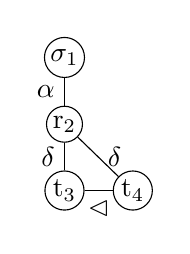
\begin{tikzpicture} [baseline = (x.base)]
\matrix (m) [matrix of nodes, column sep = 1em, row sep = 1em]{
\node[draw,circle, inner sep =1pt](x){$\sigma_{1}$}; \\
\node[draw,circle, inner sep =1pt](y){r$_{2}$}; \\
\node[draw,circle, inner sep =1pt](z){t$_{3}$}; & \node[draw,circle, inner sep =1pt](v){t$_{4}$}; \\
};
\draw (x) -- (y) node[left, pos=.5]{$\alpha$};
\draw (z) -- (y) node[left, pos=.5]{$\delta$};
\draw (v) -- (y) node[right, pos=.5]{$\delta$};
\draw (z) -- (v) node[below, pos=.5]{$\vartriangleleft$};
\end{tikzpicture}
\hspace{2cm}
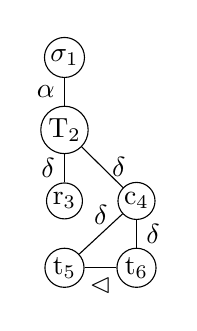
\begin{tikzpicture} [baseline = (x.base)]
\matrix (m) [matrix of nodes, column sep = 1em, row sep = 1em]{
\node[draw,circle, inner sep =1pt](x){$\sigma_{1}$}; \\
\node[draw,circle, inner sep =1pt](y){T$_{2}$}; \\
\node[draw,circle, inner sep =1pt](z){r$_{3}$}; & \node[draw,circle, inner sep =1pt](v){c$_{4}$}; \\
\node[draw,circle, inner sep =1pt](q){t$_{5}$}; & \node[draw,circle, inner sep =1pt](s){t$_{6}$}; \\
};
\draw (x) -- (y) node[left, pos=.5]{$\alpha$};
\draw (z) -- (y) node[left, pos=.5]{$\delta$};
\draw (v) -- (y) node[right, pos=.5]{$\delta$};
\draw (q) -- (v) node[above, pos=.5]{$\delta$};
\draw (s) -- (v) node[right, pos=.5]{$\delta$};
\draw (q) -- (s) node[below, pos=.5]{$\vartriangleleft$};
\end{tikzpicture}
\end{center}
When translating between the models, the simplest approach seems to be to preserve the ordering relation on these elements. A rising tone in Yip's model becomes a rising tone in Bao's model, a falling translates to a falling. Our current definition prevents this, as terminal nodes in the output (which need an order) are equivocated with register and `c' nodes, which have no apparent order. This begs the question: why not define terminal nodes in the output model in terms of those in the input model? Such an approach results in a slender, uncomplicated model.
\begin{equation}
\begin{split}
P^{\Gamma}_{\sigma}(x) &\myeq P_{\sigma}(x) \\
P^{\Gamma}_{rf}(x) &\myeq P_{T}(x) \\
P^{\Gamma}_{cf}(x) &\myeq P_{cf}(x) \\
\alpha^{\Gamma}(x)=y &\myeq \alpha(x)\\
\delta^{\Gamma}(x)=y &\myeq \varphi(x,y)\,|\,P_{cf}(x)\land P_{T}(y) \\
\mathtt{succ}^{\Gamma}(x)=y &\myeq \mathtt{succ}(x)
\end{split}
\end{equation}
The intuitive statement made by the transduction is simply: `Yip's register node is structurally equivalent to Bao's `T' node, and featurally equivalent to Bao's register node'. Everything else stays the same.
\begin{center}
\begin{tikzpicture}[baseline = (m-2-1.base)]
\matrix (m) [matrix of nodes, nodes={circle, draw, minimum size = .7cm}, column sep = .2cm, row sep = .6cm]{
& $\sigma_{1}$ & \\
& T$_2$ & \\
rf$_3$ & & c$_4$\\
cf$_5$ & & cf$_6$\\
};
\draw [->] (m-1-2.south) -- (m-2-2.north) node[left, pos=.5]{$\alpha(x)$}; 
\draw [->] (m-3-1.north) -- (m-2-2.south west) node[left, text width=.6cm,pos=.6]{$\delta(x)$};
\draw [->] (m-3-3.north) -- (m-2-2.south east) node[right, text width=.6cm,pos=.6]{$\delta(x)$};
\draw [->] (m-4-3.north) -- (m-3-3.south) node[right, text width=.6cm,pos=.5]{$\delta(x)$};
\draw [->] (m-4-1.north) -- (m-3-3.south west) node[below, pos=.6]{$\delta(x)$};
\draw [->] (m-4-1.east) -- (m-4-3.west) node[below, pos=.5]{$\vartriangleleft$};
\end{tikzpicture}
\hspace{.5cm}
$\rightarrow$
\hspace{.5cm}
\begin{tikzpicture} [baseline = (m-2-1.base)]
\matrix (m) [matrix of nodes, nodes={circle, draw, minimum size=.7cm}, column sep = .2cm, row sep = .6cm]{
& $\sigma^{\Gamma}_{1}$ & \\
& rf$^{\Gamma}_2$ & \\
3 & & 4\\
cf$^{\Gamma}_5$&&cf$^{\Gamma}_6$\\
};
\draw [->] (m-1-2.south) -- (m-2-2.north) node[right, pos=.5]{$\alpha^{\Gamma}(x)=y$}; 
\draw [->] (m-4-1.north) -- (m-2-2.south) node[right, pos=.5]{$\delta^{\Gamma}(x)$};
\draw [->] (m-4-3.north) -- (m-2-2.south);
\draw [->] (m-4-1.east) -- (m-4-3.west) node[below, pos=.5]{$\vartriangleleft$};
\end{tikzpicture}
\end{center} \par
But does this generalize to the Yip-to-Bao transduction? Yes. Here, we define an equivalency between the $P_{cf}$ nodes in the input and the $P_{cf}$ (terminal tonal) nodes in the \emph{second copy set} of the output, as well as the successor function therein. The tonal root `T' is equivalent to the register node in the first copy set. Register and `c' nodes correspond to TBU and register nodes of the second copy set.
\begin{center}
\begin{tikzpicture} [baseline = (m-2-1.base)]
\matrix (m) [matrix of nodes, nodes={circle, draw, minimum size=.7cm}, column sep = .2cm, row sep = .4cm]{
&$\sigma_{1}$& \\
&rf$_{2}$& \\
cf$_{3}$& & cf$_{4}$ \\
};
\draw [->] (m-1-2.south) -- (m-2-2.north) node[left, pos=.5]{$\alpha(x)$};
\draw [->] (m-3-1.north) -- (m-2-2.south west) node[left, text width=.6cm,pos=.6]{$\delta(x)$};
\draw [->] (m-3-3.north) -- (m-2-2.south east) node[right, text width=.6cm,pos=.6]{$\delta(x)$};
\draw [->] (m-3-1.east) -- (m-3-3.west) node[below, pos=.5]{$\vartriangleleft$};
\end{tikzpicture}
\hspace{1cm}
$\rightarrow$
\hspace{1cm}
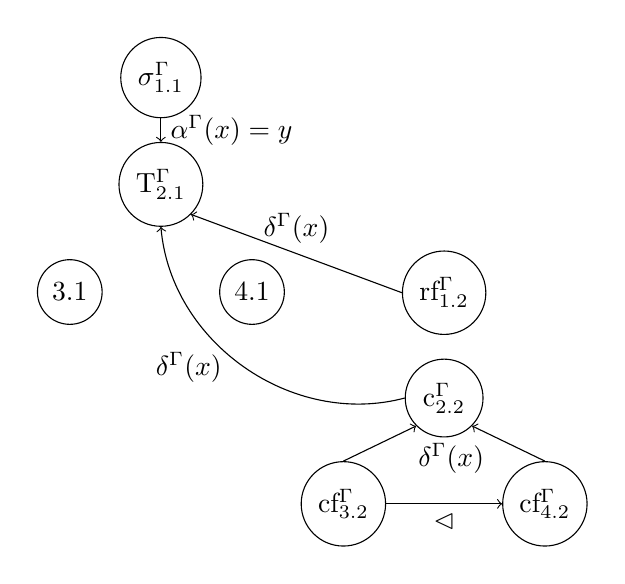
\begin{tikzpicture} [baseline = (m-2-2.base)]
\matrix (m) [matrix of nodes, nodes={circle, draw, minimum size=.7cm}, column sep = .2cm, row sep = .3cm]{
&$\sigma^{\Gamma}_{1.1}$& \\
&T$^{\Gamma}_{2.1}$& \\
3.1 & & 4.1 & & rf$^{\Gamma}_{1.2}$\\
& & & & c$^{\Gamma}_{2.2}$ \\
& & & cf$^{\Gamma}_{3.2}$ & & cf$^{\Gamma}_{4.2}$\\
};
\draw [->] (m-1-2.south) -- (m-2-2.north) node[right, pos=.5]{$\alpha^{\Gamma}(x)=y$};
\draw [->] (m-3-5.west) -- (m-2-2.south east) node[above, pos=.5]{$\delta^{\Gamma}(x)$};
\path [->, bend left=50] (m-4-5.west) edge node[left, text width=1cm, pos=.5]{$\delta^{\Gamma}(x)$} (m-2-2.south);
\draw [->] (m-5-4.north) -- (m-4-5.south west);
\draw [->] (m-5-6.north) -- (m-4-5.south east) node[left, text width = 1.4cm, pos=.09]{$\delta^{\Gamma}(x)$};
\draw [->] (m-5-4.east) -- (m-5-6.west) node[below, pos=.5]{$\vartriangleleft$};
\end{tikzpicture}
\end{center} 
\newpage
Or, more explicitly:
\begin{equation}
\begin{aligned}
P^1_{\sigma}(x) &\myeq P_{\sigma}(x) &  P^2_{\sigma}(x) &\myeq \mathtt{False} \\
P^1_{T}(x) &\myeq P_{rf}(x) &  P^2_{T}(x) &\myeq \mathtt{False} \\
P^1_{rf}(x) &\myeq \mathtt{False} &  P^2_{rf}(x) &\myeq P_{\sigma}(x) \\
P^1_{c}(x) &\myeq \mathtt{False} &  P^2_{c}(x) &\myeq P_{rf}(x) \\
P^1_{cf}(x) &\myeq \mathtt{False} &  P^2_{cf}(x) &\myeq P_{cf}(x) \\
\alpha^{1,1}(x)=y &\myeq \alpha(x) & \alpha^{1,2}(x)=y &\myeq \mathtt{False}  \\
\alpha^{2,1}(x)=y &\myeq \mathtt{False} & \alpha^{2,2}(x)=y &\myeq \mathtt{False}  \\
\mathtt{succ}^{1,1}(x) = y &\myeq \mathtt{False} & \mathtt{succ}^{1,2}(x) = y &\myeq \mathtt{False} \\
\mathtt{succ}^{2,1}(x) = y &\myeq \mathtt{False} & \mathtt{succ}^{2,2}(x) = y &\myeq \mathtt{succ}(x) \\
\delta^{1,1}(x)=y &\myeq \mathtt{False} & \delta^{1,2}(x)=y &\myeq \mathtt{False}  \\
\delta^{2,1}(x)=y &\myeq \varphi(x,y)\,|\,\Big(P_{rf}(x) \wedge P_{\sigma}(y)\Big)\,\lor & \delta^{2,2}(x)=y &\myeq \delta(x)\\
&\qquad \qquad \ \ \ \Big(P_{cf}(x) \wedge P_{\sigma}(y)\Big)\\
\end{aligned}
\end{equation}
The general transduction captures a number of important intuitions about how Bao's model relates to Yip's model. One is the equivalence between Bao's `T' and Yip's register node (that is, the tonal root), which is defined on $P_{T}$ the first copy set. Note that the inverse was defined in $\Gamma_{\text{yb}}$. There is also a parallel correlation between the Bao's `c' and Yip's register node, that being the node which dominates the tonal terminals. This relation is defined over \emph{the second copy set}, thus allowing Yip's register node to occupy different structural roles in Bao's terms simultaneously. With the `c' node in the second copy set, terminal labels, order, and c$\rightarrow$t dominance can all be defined within the second copy set. Deriving the dominance relations between the `extra' pieces of structure in Bao's model (T dominates c, T dominates r) is achieved through defining $\delta(x)$ between the second and first copy sets. 
\end{document}

